    We show a somewhat suboptimal but simple construction. A $t$-nice
    polygon has at most $t$ edges.  Let $\psi$ be the sensitivity of
    $\Body$, and place a minimum set of points $\PS$ on the boundary
    of $\Body$, which includes all the vertices of $\Body$, and such
    that the distance between any consecutive pair of points is in the
    range $[\constA, 2\constA]$, where
    $\constA = \epsA \psi/ \constB$, for some sufficiently large
    constant $\constB$. In particular, let
    $M =\max_{e \in \EGX{\Body}} \ceil{\| e\| / \constA} = \Of(
    1/\epsA)$.

    In addition, place $\constC \cdot t$ equally spaced points between
    any two consecutive points of $\PS$, where $\constC$ is a constant
    to be determined shortly. Let $\PSA$ be the set resulting from
    $\PS$ after adding all these points.

    \begin{figure}[h]
        \phantom{}%
        \hfill%
        \includegraphics[page=2,width=0.3\linewidth]{../figs/decompose}
        \hfill%
        \includegraphics[page=3,width=0.3\linewidth]{../figs/decompose}
        \hfill%
        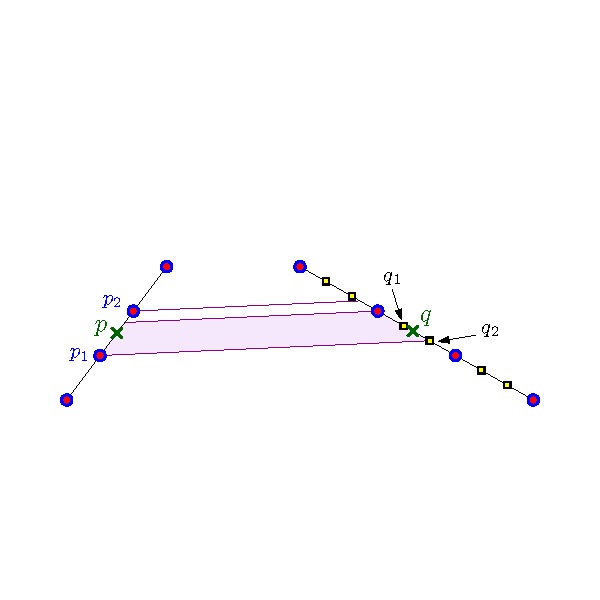
\includegraphics[page=1,width=0.3\linewidth]{../figs/points_trap}
        \hfill%
        \phantom{}%
        \caption{The points of $\PS$ (round), and all the points added
           to $\PS$ in order to create $\PSA$ (square). On the right,
           a ``vertical'' decomposition induced by one of the
           directions of $\PS \times \PSA$.}
        \figlab{v:decompose}
    \end{figure}

    We have that $|\PS| = \Of( t /\epsA)$ and
    $|\PSA| = \Of(t^2/\epsA)$. For a direction $v$, let $\Traps_v$ be
    the decomposition into trapezoids formed by shooting rays from
    inside $\Body$ in the direction of $v$ (or $-v$) from all the
    points of $\PS$, see \figref{v:decompose}. Let $\Traps_v'$ be the
    set resulting from throwing away trapezoids with legs that lie on
    adjacent edges.  It is easy to verify that all the trapezoids of
    $\Traps_v'$ are $\epsA$-narrow.  Let $U$ be the set of all
    directions induced by pairs of points of $\PS \times \PSA$, and
    let $\Traps = \cup_{u \in U} \Traps_u'$. We have that
    $|\Traps| = \Of( |\PS| \cdot |U| ) = \Of(|\PS|^2 |\PSA| ) =\Of(
    t^4 /\epsA^3)$.

    Consider any two points $\pa, \pb$ on non-adjacent edges of
    $\Body$, and let $\pa_1, \pa_2 $ be the two adjacent points of
    $\PS$ such that $\pa \in \pa_1 \pa_2$.  Now, let $\pb_1, \pb_2$ be
    the adjacent points of $\PSA$ such that $\pb \in \pb_1 \pb_2$.  We
    assume that $\pa_1, \pa_2, \pb_1,\pb_2$ are in this clockwise
    order along the boundary of $\Body$.

    Observe that when we project the interval $\pa_1 \pa_2$, to the
    line induced by $\pb_1 \pb_2$, in the direction
    $\overrightarrow{\pa_1 \pb_2}$, the projected interval contains
    $\pb_1 \pb_2$.  The last claim is intuitively obvious, but
    requires some work to see formally. The minimum height of a
    triangle involving three vertices of $\Body$ is formed by three
    consecutive vertices. In the worst case, this is an isosceles
    triangle with sidelength $\psi$ and base angle $\pi/t$. As such,
    the height of such a triangle is
    $h = \psi \sin( \pi/t) \geq \psi/t$.


    \begin{figure}[h]
        \includegraphics[page=2,width=0.23\linewidth]{../figs/points_trap_2}%
        \hfill%
        \includegraphics[page=3,width=0.23\linewidth]{../figs/points_trap_2}
        \hfill%
        \includegraphics[page=4,width=0.23\linewidth]{../figs/points_trap_2}
        \hfill%
        \includegraphics[page=5,width=0.23\linewidth]{../figs/points_trap_2}
        \caption{The height of the triangle
           $\triangle \pa_1 \pa_2 \pb_2$ is minimized as $\pb_2$ and
           $\pa_1$ are moved to vertices of $\Body$.}%
        \figlab{points:move}
    \end{figure}

    The height of the triangle $\triangle \pa_1 \pa_2 \pb_2$ is
    minimized when $\pa_1$ or $\pa_2$ is a vertex of $\Body$, and
    $\pb_2$ is at a vertex of $\Body$, see
    \figref{points:move}. Assume, for concreteness, that $\pa_1$ is a
    vertex of $\Body$, and observe that
    $\dY{\pa_1}{\pa_2} \geq \| e\|/M$, where $e$ is the edge of
    $\Body$ containing this segment. Using similar triangles, it is
    straightforward to show that the height of this triangle is at
    least $h' = h/M = \Omega( \eps \psi/t )$. The quantity $h'$ is a
    lower bound on the length of the projection of $\pa_1 \pa_2$ on
    the line spanned by $\pb_1 \pb_2$. However,
    $\dY{\pb_1}{\pb_2} \leq 2\constA/\constC t = \Of( \epsA \psi
    /\constC t) < h'$, by picking $\constC$ to be a sufficiently large
    constant.

    This readily implies that the trapezoid induced by the direction
    $ u = \overrightarrow{\pa_1 \pb_2}$ in $\Traps_u'$ that contains
    $\pa$ on one of its leg, and $\pb$ on the other.
